\chapter{Resultados}
\label{chap:resultados}

	Neste capítulo, são apresentadas as avaliações da projeção e da visualização como
	instrumento para avaliação de programas, ambos considerando um conjunto de
	programas escritos em Python para uma disciplina introdutória à Computação.
	
	
	\section{Descrição da base}
	\label{sec:resultados:base-apoo}

		Essa base é constituída de 152 implementações em Python de 5 problemas distintos.
		Os desenvolvedores das implementações foram anonimizados, sendo representados por 
		sequências de números. Os problemas tratados foram os seguintes. O primeiro exercício
		consiste na revisão de conceitos básicos como: estruturas de condição e laço de repetição. O
		segundo exercício define a criação de classes com mais de um construtor, e manipulação de
		arquivos e cadeia de caracteres. O terceiro exercício consiste na criação das classes
		\texttt{Palavra} e \texttt{Texto}, no qual a primeira classe deve ser utilizada na segunda
		classe, e uma classe para gerar orações gramaticais. O quarto exercício refere-se a
		utilização de herança e polimorfismo, identificando cada palavra contida em um arquivo. O
		quinto exercício consiste na alteração de uma classe, implementando sobreposição de
		operadores. 
		
	
	\section{Avaliação da projeção com preservação de vizinhança}

	A \foreign{ScienceView} utiliza a preservação da vizinhança
	(\cref{subsubsec:vizinhanca}) para verificar a qualidade das projeções. A \cref{fig:neighborhoodAPOO30}
	apresenta a qualidade da projeção para essa base de dados. Essa técnica visa avaliar
	se houve uma preservação da vizinhança dos objetos no espaço de alta dimensionalidade
	na projeção. A \foreign{Neighborhood Preservation} é calculada tomando os $k$ vizinhos
	mais próximos de uma instância no espaço de alta dimensionalidade e os $k$ vizinhos
	mais próximos na projeção, e verificando-se que proporção da vizinhança é preservada
	na projeção. A precisão final para um dado valor de $k$ é a média das precisões para
	cada instância. Esse cálculo é feito para vários valores de $k$ (tipicamente $k=[2,...,30]$)
	de forma a obtermos uma curva. Quanto mais altos os valores da curva para cada valor
	de $k$, maior a qualidade da projeção. Considerando que a técnica \acl{T-LSP} \cite{Alencar}
	gera uma sequência de projeções, temos uma curva para cada projeção da
	sequência.
	
	Observa-se a precisão de 20\% para a linha (\texttt{year} $5$, obtida com 30 vizinhos para a
	projeção considerando todos os problemas (e, consequentemente, todas as submissões). Considerando
	outros trabalhos que utilizam esta medida para avaliação de qualidade de projeções~\cite{phd:paulovich},
	a qualidade da projeção é adequada e compatível com outras projeções feitas com a técnica LSP e
	similares.
	
	
	Na \cref{fig:neighborhoodAPOO30} é possível observar que as projeções no início da
	sequência apresentam menor qualidade quando comparada as demais, como é possível observar
	nas curvas dos problemas $3$, $4$ e $5$. Também é
	possível notar que a projeção perde um pouco mais que $12\%$ de informação para as
	projeções dos anos $4$ e $5$ considerando a comparação de $15$ vizinhos do espaço
	$n$-dimensional com o espaço bidimensional.
	
	
	\begin{figure}
		\centering
		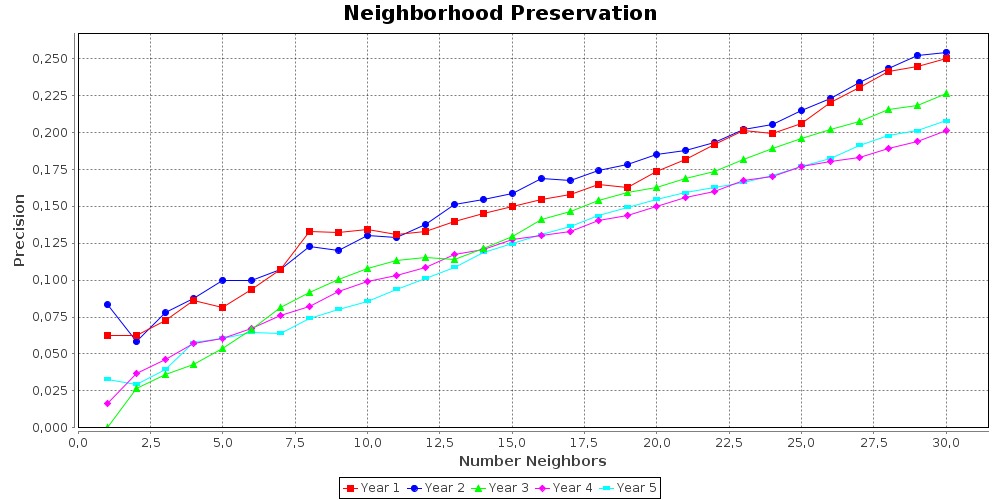
\includegraphics[width=0.7\linewidth]{imagem/neighborhoodAPOO30}
		\caption{Qualidade da projeção, utilizando a preservação de vizinhança (\foreign{neighborhood preservation})}
		\label{fig:neighborhoodAPOO30}
	\end{figure}	

	
	\section{Avaliação qualitativa da visualização}
	\label{sec:avalQualitativa}
	
		Para obter resultados qualitativos dessa pesquisa, realizamos um estudo experimental com
		as seguintes etapas: treinamento, utilização e questionário.
		
		% TODO: como foram organizadas as pessoas, quantas pessoas, os tempos
		
		O treinamento foi realizado na forma de tutorial com a apresentação dos critérios
		de avaliação (estilo de escrita e complexidade ciclomática) e da ferramenta com
		duração de $55$ minutos. Especificamente quanto à ferramenta, foram apresentados
		todos os passos referentes ao seu funcionamento, desde a inserção de uma nova
		coleção no banco de dados até a visualização das implementações com a visualização
		da projeção criada a partir da coleção. Em seguida, foi apresentado como utilizar
		a ferramenta para auxiliar na avaliação das implementações: visualizar os
		agrupamentos formados ao longo das projeções, selecionar um determinado conjunto
		de implementações, identificar as características semelhantes de tais grupos e
		abrir mais de uma implementação simultaneamente. Durante o treinamento, foi utilizada uma
		base de dados distinta da descrita na \cref{sec:resultados:base-apoo}.
		
		% TODO: informar que eles tiveram 20 minutos para avaliar trabalhos. 
		% TODO: falar quantas pessoas foram e como elas foram organizados (dois grupos: primeiramente, um grupo avaliou de forma tradicional, com auxílio dos dados obtidos pela ScienceView-Python e o outro grupo avaliou com auxílio da ferramenta. Depois foram invertidas as intervenções. Em ambos os casos, a cada rodada de avaliações, cada participante criou um relato sobre os programas avaliados e comentários que seriam enviados para os alunos, considerando os erros identificados.)
		Encerrado o treinamento, procedeu-se para a utilização da ferramenta com a base
		descrita na \cref{sec:resultados:base-apoo}. Para iniciarmos essa etapa, foi
		pedido para que os participantes encerrassem o funcionamento da \foreign{ScienceView}
		e a executassem com a criação da base de dados. O experimento teve participação
		de $4$ pessoas e ambos os grupos utilizaram os dados obtidos pela \foreign{ScienceView-Python}
		\cref{sec:scienceView-Python}. Todos os contribuintes realizaram  correção manual,
		o qual consistiu na correção somente do código-fonte sem utilizar a ferramenta, e
		somente $3$ pessoas utilizaram a ferramenta \foreign{ScienceView} para auxiliar
		na correção. O experimento consistiu em duas etapas. Na primeira etapa, $1$
		voluntário realizou a correção manual, enquanto os outros $2$, utilizaram a
		ferramenta para auxiliar na correção com duração de $20$ minutos. Na segunda
		etapa, o contribuinte que realizou a correção manual, passou a utilizar a
		\foreign{ScienceView}, enquanto os $2$ que utilizaram a ferramenta na etapa
		anterior, realizaram a correção manual durante $22$ minutos. Os participantes
		utilizaram a ferramenta sem ajuda no que já tinha sido apresentado e o
		avaliaram por meio de um questionário.		
		
		O questionário (\cref{apendice:questionario}) apresenta questões objetivas e
		dissertativas para avaliar a qualidade do treinamento e da ferramenta. Enquanto
		as questões objetivas visavam a qualidade do treinamento, da ferramenta e se
		é possível utilizá-la para auxiliar na correção, as questões dissertativas
		visam a encontrar lacunas observadas pelo participante para uma possível 
		atualização da ferramenta.
		
		A \cref{fig:projecaoFinal} apresenta a visualização dos agrupamentos das 152
		implementações contidas na base de dados. Isso foi possível após a adaptação da
		ferramenta para leitura de arquivos no formato \texttt{CSV}. Cada ponto da
		visualização é referente a um código-fonte. Ao clicar em um dos pontos,
		uma interface exibe sua implementação e as características extraídas pela
		\foreign{ScienceView-Python} para aquele código-fonte. Também é possível ordenar
		as colunas de características \foreign{Quantity} e \foreign{Normalized} em
		ordem  crescente ou decrescente para visualizar as características que mais
		ocorreram. Por padrão, a tabela é apresentado ordenada de forma descrescente
		pela coluna \foreign{Normalized}.
	
		\begin{figure}[h]
			\centering
			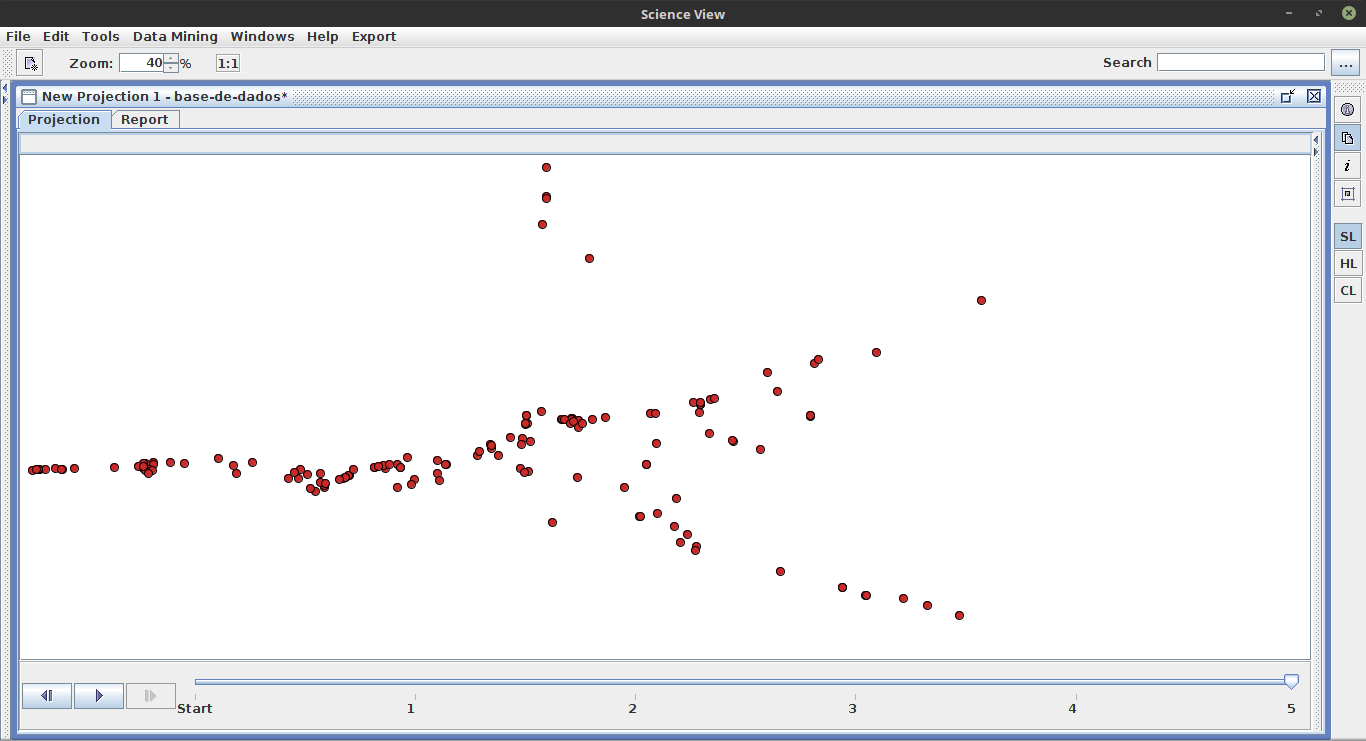
\includegraphics[width=1\linewidth]{imagem/projecaoFinal} % TODO: substituir, futuramente, pela figura da ferramenta corrigida.
			\caption[Visualização dos agrupamentos da base de dados gerado pela \texttt{ScienceView}]
			{Visualização dos agrupamentos da base de dados gerado pela \texttt{ScienceView} \cite{Alencar-etal:2012}}
			\label{fig:projecaoFinal}
		\end{figure}
		
		A \cref{tab:resultados} apresenta a quantidade de implementações que cada
		participante corrigiu e de comentários realizados. A primeira linha identifica
		qual participante realizou as correções. E a primeira coluna indica a forma
		de correção realizada pelos voluntários. Então, é apresentado a quantidade
		de correções que cada participante conseguiu realizar e a quantidade de
		comentários conforme o tipo de correção.
		
		\begin{table}[h]
			\begin{tabularx}{\linewidth}{|X|X|X|X|X|}
		        \hline
		        
		        & Voluntário 1
		        & Voluntário 2
		        & Voluntário 3
		        & Voluntário 4\\
		        
		        \hline
		        Correção tradicional
		        & 3 códigos-fontes e 2 comentários para correção do aluno
		        & 4 códigos-fontes e 3 comentários para correção do aluno
		        & 3 códigos-fontes e 2 comentários para correção do aluno
		        & 5 códigos-fontes e 2 comentários para correção do aluno\\
		        
		        \hline
		        \foreign{ScienceView}
		        & Não utilizou a ferramenta
		        & 4 códigos-fontes e 4 comentários realizados
		        & 3 códigos-fontes e observou que a ferramenta auxiliou no encontro dos erros de forma mais rápida.
		        & 4 códigos-fontes e 3 comentários para correção dos alunos\\
		        \hline
			\end{tabularx}
			\caption{Quantidade de correções e comentários realizados com e sem a utilização da ferramenta}
			\label{tab:resultados}
		\end{table}
		
%		As implementações das \cref{fig:codigo1} e \cref{fig:codigo2} foram consideradas
%		semelhantes, devido aos seus respectivos pontos estarem próximos no mapa de
%		projeção. É possível notar que há diversas semelhanças nos tipos das características
%		extraídas e erros que ocorreram pela coluna \foreign{Normalized}, além da quantidade
%		dessas características apresentadas na coluna \foreign{Quantity}.
%		
%		\begin{figure}[h]
%			\centering
%			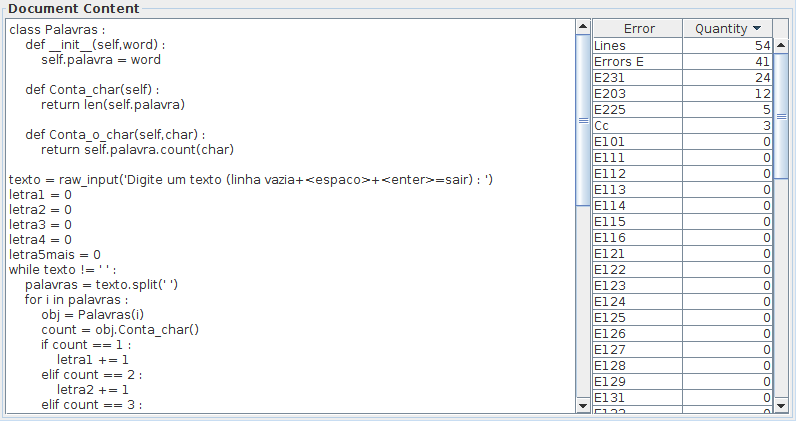
\includegraphics[width=0.8\linewidth]{imagem/codigo1}
%			\caption[Representação parcial da interface que apresenta o código e suas características]
%			{Representação parcial da interface que apresenta o código e suas características \cite{Alencar-etal:2012}}
%			\label{fig:codigo1}
%		\end{figure}
%		
%		\begin{figure}[H]
%			\centering
%			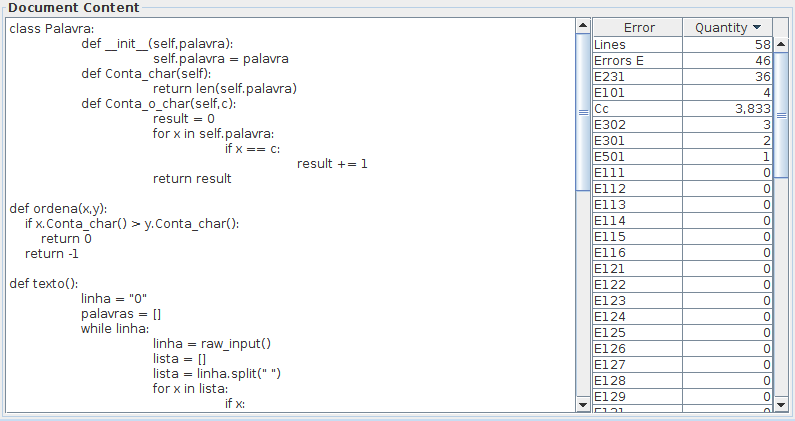
\includegraphics[width=0.8\linewidth]{imagem/codigo2}
%			\caption[Representação parcial da interface que apresenta o código considerado semelhante ao da \cref{fig:codigo1}]
%			{Representação parcial da interface que apresenta o código considerado semelhante ao da \cref{fig:codigo1} \cite{Alencar-etal:2012}}
%			\label{fig:codigo2}
%		\end{figure}
		
		Para finalizar o experimentos, os voluntários, responderam o questionário (\cref{apendice:questionario})
		anonimamente. A primeira questão refere-se ao tempo de experiência como professor,
		visto que acreditávamos que essa experiência poderia interferir na quantidade
		de correções realizadas com a ferramenta. Dentre eles, $2$ cooperadores possuem
		menos que $1$ ano de experiência, enquanto $1$ possui mais de $10$ anos de
		experiência como professor. E todos eles afirmaram que o treinamento em forma
		de tutorial da \foreign{ScienceView} contribui para sua utilização.
		
		Obtivemos êxito com a adaptação da interface que apresenta o código-fonte e a
		tabela de erros, visto que, ao serem questionados se faltava
		alguma informação nessa interface, todos responderam negativamente.
		
		Apesar dos $3$ voluntários afirmarem que a \foreign{ScienceView} colaborou
		para a correção das implementações, $2$ deles corrigiram a mesma quantidade
		de implementações utilizando a ferramenta e manualmente. A exceção ocorreu com 
		apenas $1$ participante que extraiu os tópicos semelhantes manualmente. Na
		primeira extração, selecionou apenas $2$ códigos-fontes e observou que os
		erros apresentados na tabela de erros eram semelhantes, visto que observou
		a importação de bibliotecas entre funções ao invés de realizá-las no início
		da implementação. Na segunda extração, selecionou $8$ códigos-fontes e constatou
		que os erros ocorreram nas implementações e foi compreendido corretamente
		pela ferramenta.
		
		Ao relatarem sobre o \foreign{feedback} recebido da \foreign{ScienceView}
		por meio da visualização dos agrupamentos, $2$ participantes afirmaram que
		os agrupamentos auxiliaram na verificação de implementações com características
		similares. O outro participantes constatou a possibilidade de utilizar a
		ferramenta em uma turma fechada de alunos a fim de verificar quais os principais
		erros deles por meio da extração de tópicos da ferramenta.
		
		Sobre a experiência em relação ao uso da ferramenta, um dos participantes
		admite que, como não utilizou muito a ferramenta, foi mais rápido realizar
		as correções manuais. Contudo, outra resposta afirma que a utilização mais
		frequente da \foreign{ScienceView}, evidenciará analisar as implementações
		de forma mais rápida.
		
		
% TODO: deixar para artigo
%	
%	\section{Projeção e visualização de MIT 6.00.1x}	
%
%	\subsection{Descrição da base}
%	% TODO: descrever base de dados: quais foram os tipos de programas, quantos foram, falar que a
%	% base não foi anonimizada porque os programas estavam publicamente disponíveis no GitHub.
%	Essa base de dados é constituída de 3470 implementações referente a 10 exercícios
%	distintos. Todos as atividades solicitam manipulação de arquivo e cadeia de caracteres.
%	
%	O primeiro exercício requer conceitos de matriz, utilizando lista dentro
%	de lista, e programação dinâmica para solucionar o transporte de animais.
%	
%	O segundo exercício necessita de conhecimento sobre aleatoriedade, lista, condicional,
%	cadeia de caracteres, operações aritméticas e lógicas para implementar o jogo da
%	forca.
%	
%	O terceiro exercício solicita a utilização de laço de repetição, condicional, lista,
%	operações aritméticas e lógicas para implementar o jogo das palavras.
%	
%	O quarto exercício requer conhecimento de lista e dicionário pra codificar e
%	decodificar um texto.
%	O quinto exercício requer o uso de analisador (\foreign{parser}), construção
%	de classe, interface, polimorfismo e operadores lógicos para desenvolver um programa
%	de monitoramento de novos \foreign{feeds} na Internet.
%	
%	O sexto exercício solicita conhecimento sobre criação de classes, matriz, laço de
%	repetição e manipulação de interface gráfica para implementar um aspirador de pó
%	inteligente e sua simulação.
%	
%	O sétimo exercício consiste no uso de classes, aleatoriedade, laço de repetição,
%	condicional, lista e conhecimento de estatística para implementar uma simulação
%	e um sistema de tratamento de pacientes conforme o vírus que eles possuem.
%	
%	O oitavo problema consiste na implementação de classes a partir do exercício $7$.
%	Pedindo a implementação da classe \texttt{ResistantVirus} e \texttt{SimplePatient}
%	para realizar simulações desses vírus em pacientes.
%	
%	O nono exercício requer o uso de dicionário e operador lógico para desenvolver
%	um software que apresente uma lista de assuntos para cada aluno da universidade.
%	
%	E para o décimo exercício, é necessário conhecer um algoritmo de agrupamento para
%	realizar sua implementação.
%	
%	Os desenvolvedores dessas implementações não foram anonimizados, pois seus
%	códigos-fontes estavam presentes em repositórios públicos no GitHub \cite{github}.
%	
%	% TODO: Marco: colocar a string utilizada para buscar os programas e como foi criada a base
%	
%
%\subsection{Avaliação da projeção com preservação de vizinhança}
%
%
%\subsection{Avaliação qualitativa da visualização}
%% TODO: relatar o estudo: treinamento, instruções, questionário, resultados

	\section{Ameaças a validade}
	\label{sec:ameacas}
	
		% TODO: treinamento não foi suficiente para utilização da ferramenta para avaliação
		O treinamento realizado, não foi suficiente para avaliar as implementações por meio
		da utilização da \foreign{ScienceView}, visto que um dos participantes relatou que
		a falta de conhecimento sobre a ferramenta fez com que correção manual acontecesse de
		forma mais rápida. Enquanto, outro participante observou que a ferramenta agilizará
		o processo de correção conforme aumentar a frequência de uso da ferramenta. Dado
		essas duas observações, podemos concluir que o treinamento não foi suficiente para
		capacitar todos os participantes sobre a utilização da ferramenta.
		
		% TODO: treinamento tem de deixar claro que a avaliação é quanto aos trabalhos, mas não quanto a correção dos problemas automaticamente identicados
		Durante o treinamento, não foi exposto explicitamente que, ao utilizar a \foreign{ScienceView},
		a avaliação é quanto aos códigos-fontes. Com isso, além de corrigirem as implementações,
		alguns participantes buscaram verificar se as características semelhantes apontadas
		pela extração de tópicos realmente ocorria nas implementações. E isso pode ter
		impactado na correção, devido ao tempo gasto para fazer essas verificações.
		
		% TODO: outra ameaça é quanto ao tamanho da base
		O banco de dados formado por 152 códigos-fontes que solucionam 5 problemas distintos
		é considerado pequeno. Visto que, uma das características do \ac{MOOC} é a grande
		quantidade de usuários (\foreign{massive}). Desta forma, essa base de dados não
		reflete ao montante de submissões que podem ocorrer em um \acs{MOOC}
		
		% TODO: outra ameaça é quanto a quantidade de participantes
		A aplicação do experimento somente com $4$ pessoas, e ainda, somente $3$ pessoas
		utilizarem a \foreign{ScienceView} não nos retorna nada concreto estatisticamente.
		Devido a essa quantidade, temos apenas indícios do objetivo da pesquisa. Para
		viabilizar mais participantes, é necessário, além de tempo, a disponibilidade
		de professores para participar do treinamento e utilizar a ferramenta, focando
		que o desenvolvimento do projeto pode contribuir para vossas correções, além
		de possibilitar a verificação do erro mais frequente a fim de melhorar suas
		aulas.

	\section{Considerações finais}
	
		Por meio dos resultados obtidos, a próxima Seção apresentará nossa conclusão,
		considerando tanto a análise qualitativa, quanto a quantitativa. E as ameaças
		a validade observadas.
